\documentclass[a4paper, oneside]{memoir}
\usepackage[utf8]{inputenc}
\usepackage[T1]{fontenc}
\usepackage{pifont}
\usepackage{amssymb}
\usepackage{fourier}
\usepackage[dvipsnames]{xcolor}
\usepackage{tikz}
\usepackage{pdfpages}
\usepackage[sfdefault]{roboto}
\usepackage{color}

% Styles
\tikzstyle{teamshare} = [below, text width=5.4cm, inner sep = 0.5cm, text=white, align=center]
\tikzstyle{cardtext} = [below, text width=5.9cm, inner sep = 0.25cm, text centered]
\setlrmarginsandblock{0.9cm}{*}{1}
\setulmarginsandblock{1.49cm}{*}{1}
\checkandfixthelayout[nearest]
\pagestyle{empty}

% Define Commands
\newcommand{\condition}[1]{\textbf{#1}}
\newcommand{\character}[1]{\textbf{#1}}
\newdimen\titlespacing
\titlespacing=0.15cm

% Define Seperators
\newcommand{\seperator}[1]{\\ \vspace{\titlespacing} \hrulefill {} \tiny \bfseries #1 \normalfont \normalsize \hrulefill \\ \vspace{\titlespacing}}
\newcommand{\seperatoraction}{\seperator{POWER}}
\newcommand{\seperatordescription}{\seperator{DESCRIPTION}}
\newcommand{\seperatorcondition}{\seperator{CONDITION}}
\newcommand{\seperatorwin}{\seperator{HOW TO WIN}}
\newcommand{\redwinsection}{
	\seperatorwin
	You win if \character{Santa} does not gain the \condition{humbug} condition due to the \character{Grinch} stealing Christmas.
}
\newcommand{\greenwinsection}{
	\seperatorwin
	\small You win if \character{Santa} gains the \condition{humbug} condition due to the \character{Grinch} stealing Christmas.
}
\newcommand{\titlefrom}[1]{\\ \tiny > from #1 <}

% Begin Document
\begin{document}
	
% === PAGE #01 ===
\noindent 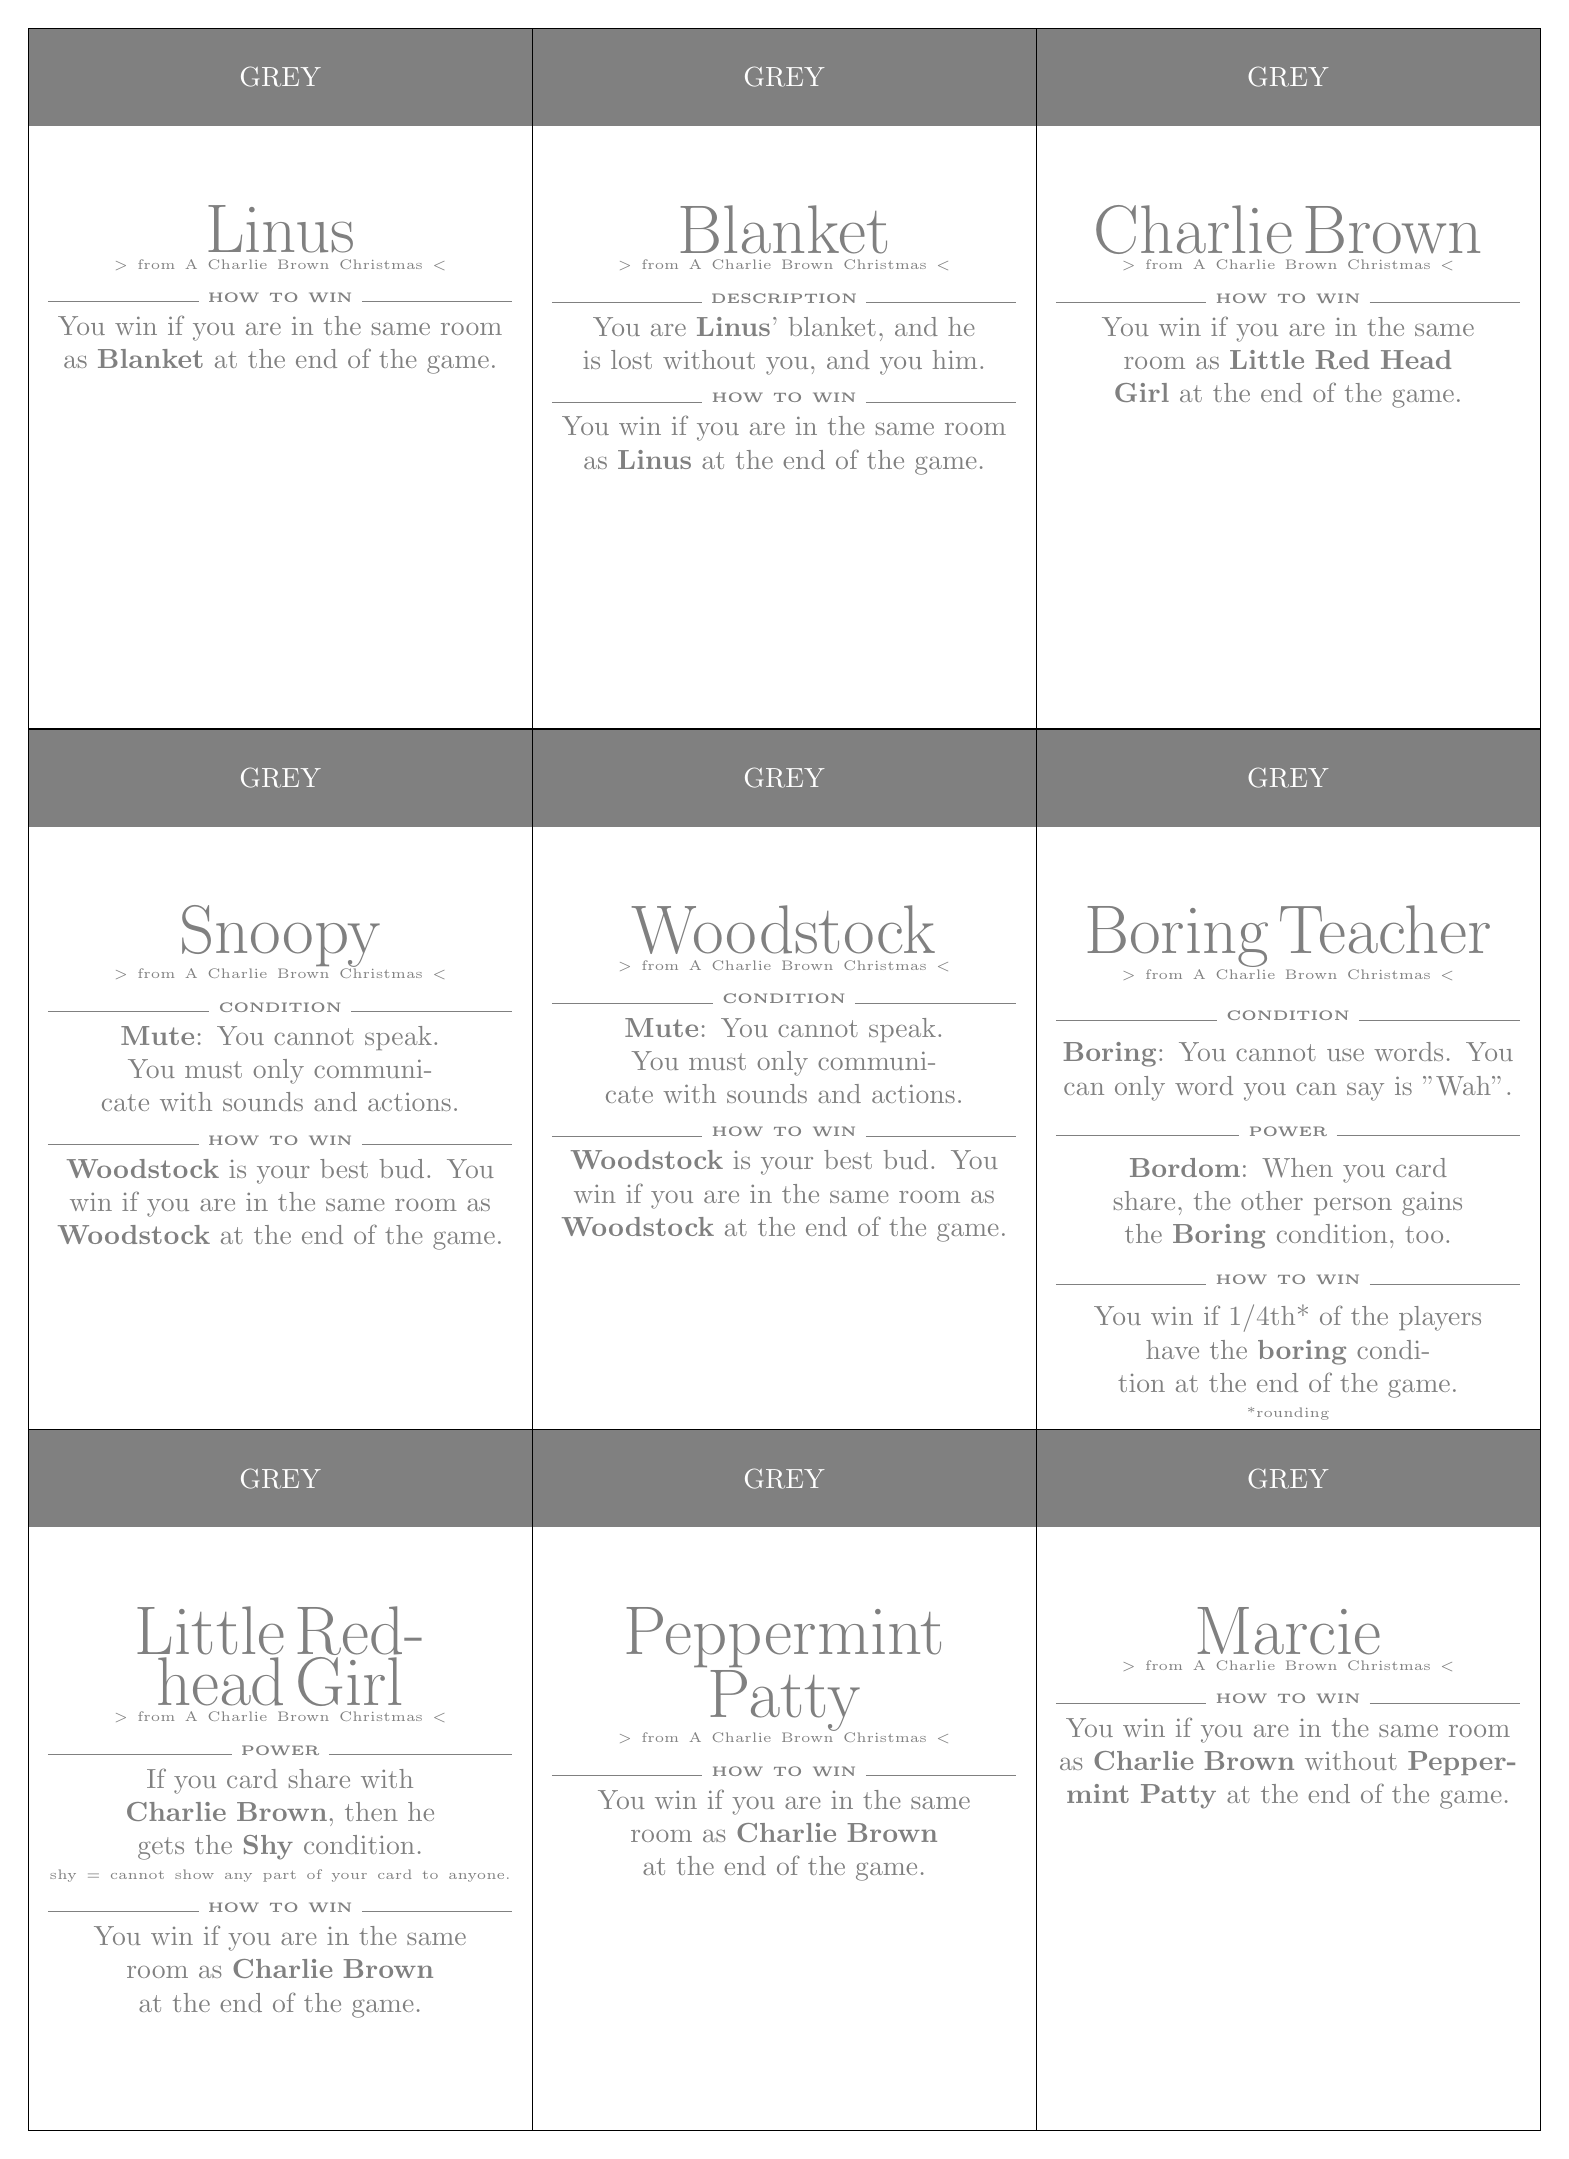
\begin{tikzpicture}[outer sep=0]

% LINUS
\node[teamshare, fill=gray] (1) at (3.2,26.7) {\HUGE GREY};
\node[cardtext, text=gray] at (3.2,24.7) {
	{\Huge Linus}
	\titlefrom{A Charlie Brown Christmas}
	\seperatorwin
	You win if you are in the same room as \character{Blanket} at the end of the game.
};

% BLANKET
\node[teamshare, fill=gray] at (9.6,26.7) {\HUGE GREY};
\node[cardtext, text=gray] at (9.6,24.7) {
	{\Huge Blanket}
	\titlefrom{A Charlie Brown Christmas}
	\seperatordescription
	You are \character{Linus}' blanket, and he is lost without you, and you him.
	\seperatorwin
	You win if you are in the same room as \character{Linus} at the end of the game.
};

% CHARLIE BROWN
\node[teamshare, fill=gray] at (16,26.7) {\HUGE GREY};
\node[cardtext, text=gray] at (16,24.7) {
	{\Huge Charlie Brown}
	\titlefrom{A Charlie Brown Christmas}
	\seperatorwin
	You win if you are in the same room as \character{Little Red Head Girl} at the end of the game.
};

% SNOOPY
\node[teamshare, fill=gray] at (3.2,17.8) {\HUGE GREY};
\node[cardtext, text=gray] at (3.2,15.8) {
	{\Huge Snoopy}
	\titlefrom{A Charlie Brown Christmas}
	\seperatorcondition
	\condition{Mute}: You cannot speak. You must only communicate with sounds and actions.
	\seperatorwin
	\character{Woodstock} is your best bud. You win if you are in the same room as \character{Woodstock} at the end of the game.
};

% WOODSTOCK
\node[teamshare, fill=gray] at (9.6,17.8) {\HUGE GREY};
\node[cardtext, text=gray] at (9.6,15.8) {
	{\Huge Woodstock}
	\titlefrom{A Charlie Brown Christmas}
	\seperatorcondition
	\condition{Mute}: You cannot speak. You must only communicate with sounds and actions.
	\seperatorwin
	\character{Woodstock} is your best bud. You win if you are in the same room as \character{Woodstock} at the end of the game.
};

% BORING TEACHER
\node[teamshare, fill=gray] at (16,17.8) {\HUGE GREY};
\node[cardtext, text=gray] at (16,15.8) {
	\titlespacing=.1cm
	{\Huge Boring Teacher}
	\titlefrom{A Charlie Brown Christmas}
	\seperatorcondition
	\condition{Boring}: You cannot use words. You can only word you can say is "Wah".
	\seperatoraction
	\condition{Bordom}: When you card share, the other person gains the \condition{Boring} condition, too.
	\seperatorwin
	You win if 1/4th* of the players \\have the \condition{boring} condition at the end of the game. \\
	\vspace{-0.1cm}
	\tiny *rounding
	\titlespacing=0.15cm
};

% LITTLE RED HEAD GIRL
\node[teamshare, fill=gray] at (3.2,8.9) {\HUGE GREY};
\node[cardtext, text=gray] at (3.2,6.9) {
	{\Huge Little Redhead Girl}
	\titlefrom{A Charlie Brown Christmas}
	\seperatoraction
	If you card share with \character{Charlie Brown}, then he gets the \condition{Shy} condition. \\
	\vspace{0.1cm}
	\tiny shy = cannot show any part of your card to anyone.
	\seperatorwin
	You win if you are in the same room as \condition{Charlie Brown} at the end of the game.
};

% PEPPERMINT PATTY
\node[teamshare, fill=gray] at (9.6,8.9) {\HUGE GREY};
\node[cardtext, text=gray] at (9.6,6.9) {
	{\Huge Peppermint Patty}
	\titlefrom{A Charlie Brown Christmas}
	\seperatorwin
	You win if you are in the same room as \condition{Charlie Brown} at the end of the game.
};

% MARCIE
\node[teamshare, fill=gray] at (16,8.9) {\HUGE GREY};
\node[cardtext, text=gray] at (16,6.9) {
	{\Huge Marcie}
	\titlefrom{A Charlie Brown Christmas}
	\seperatorwin
	You win if you are in the same room as \condition{Charlie Brown} without \character{Peppermint Patty} at the end of the game.
};


\draw (0,0) -- (19.2,0);
\draw (0,8.9) -- (19.2,8.9);
\draw (0,17.8) -- (19.2,17.8);
\draw (0,26.7) -- (19.2,26.7);

\draw (0,0) -- (0,26.7);
\draw (6.4,0) -- (6.4,26.7);
\draw (12.8,0) -- (12.8,26.7);
\draw (19.2,0) -- (19.2,26.7);



\end{tikzpicture}

%Background is not my own. But courtesy of a user on BGG

\includepdf[pages={1}, angle=90]{cardsbackground.pdf}




% === PAGE #02 ===
\noindent 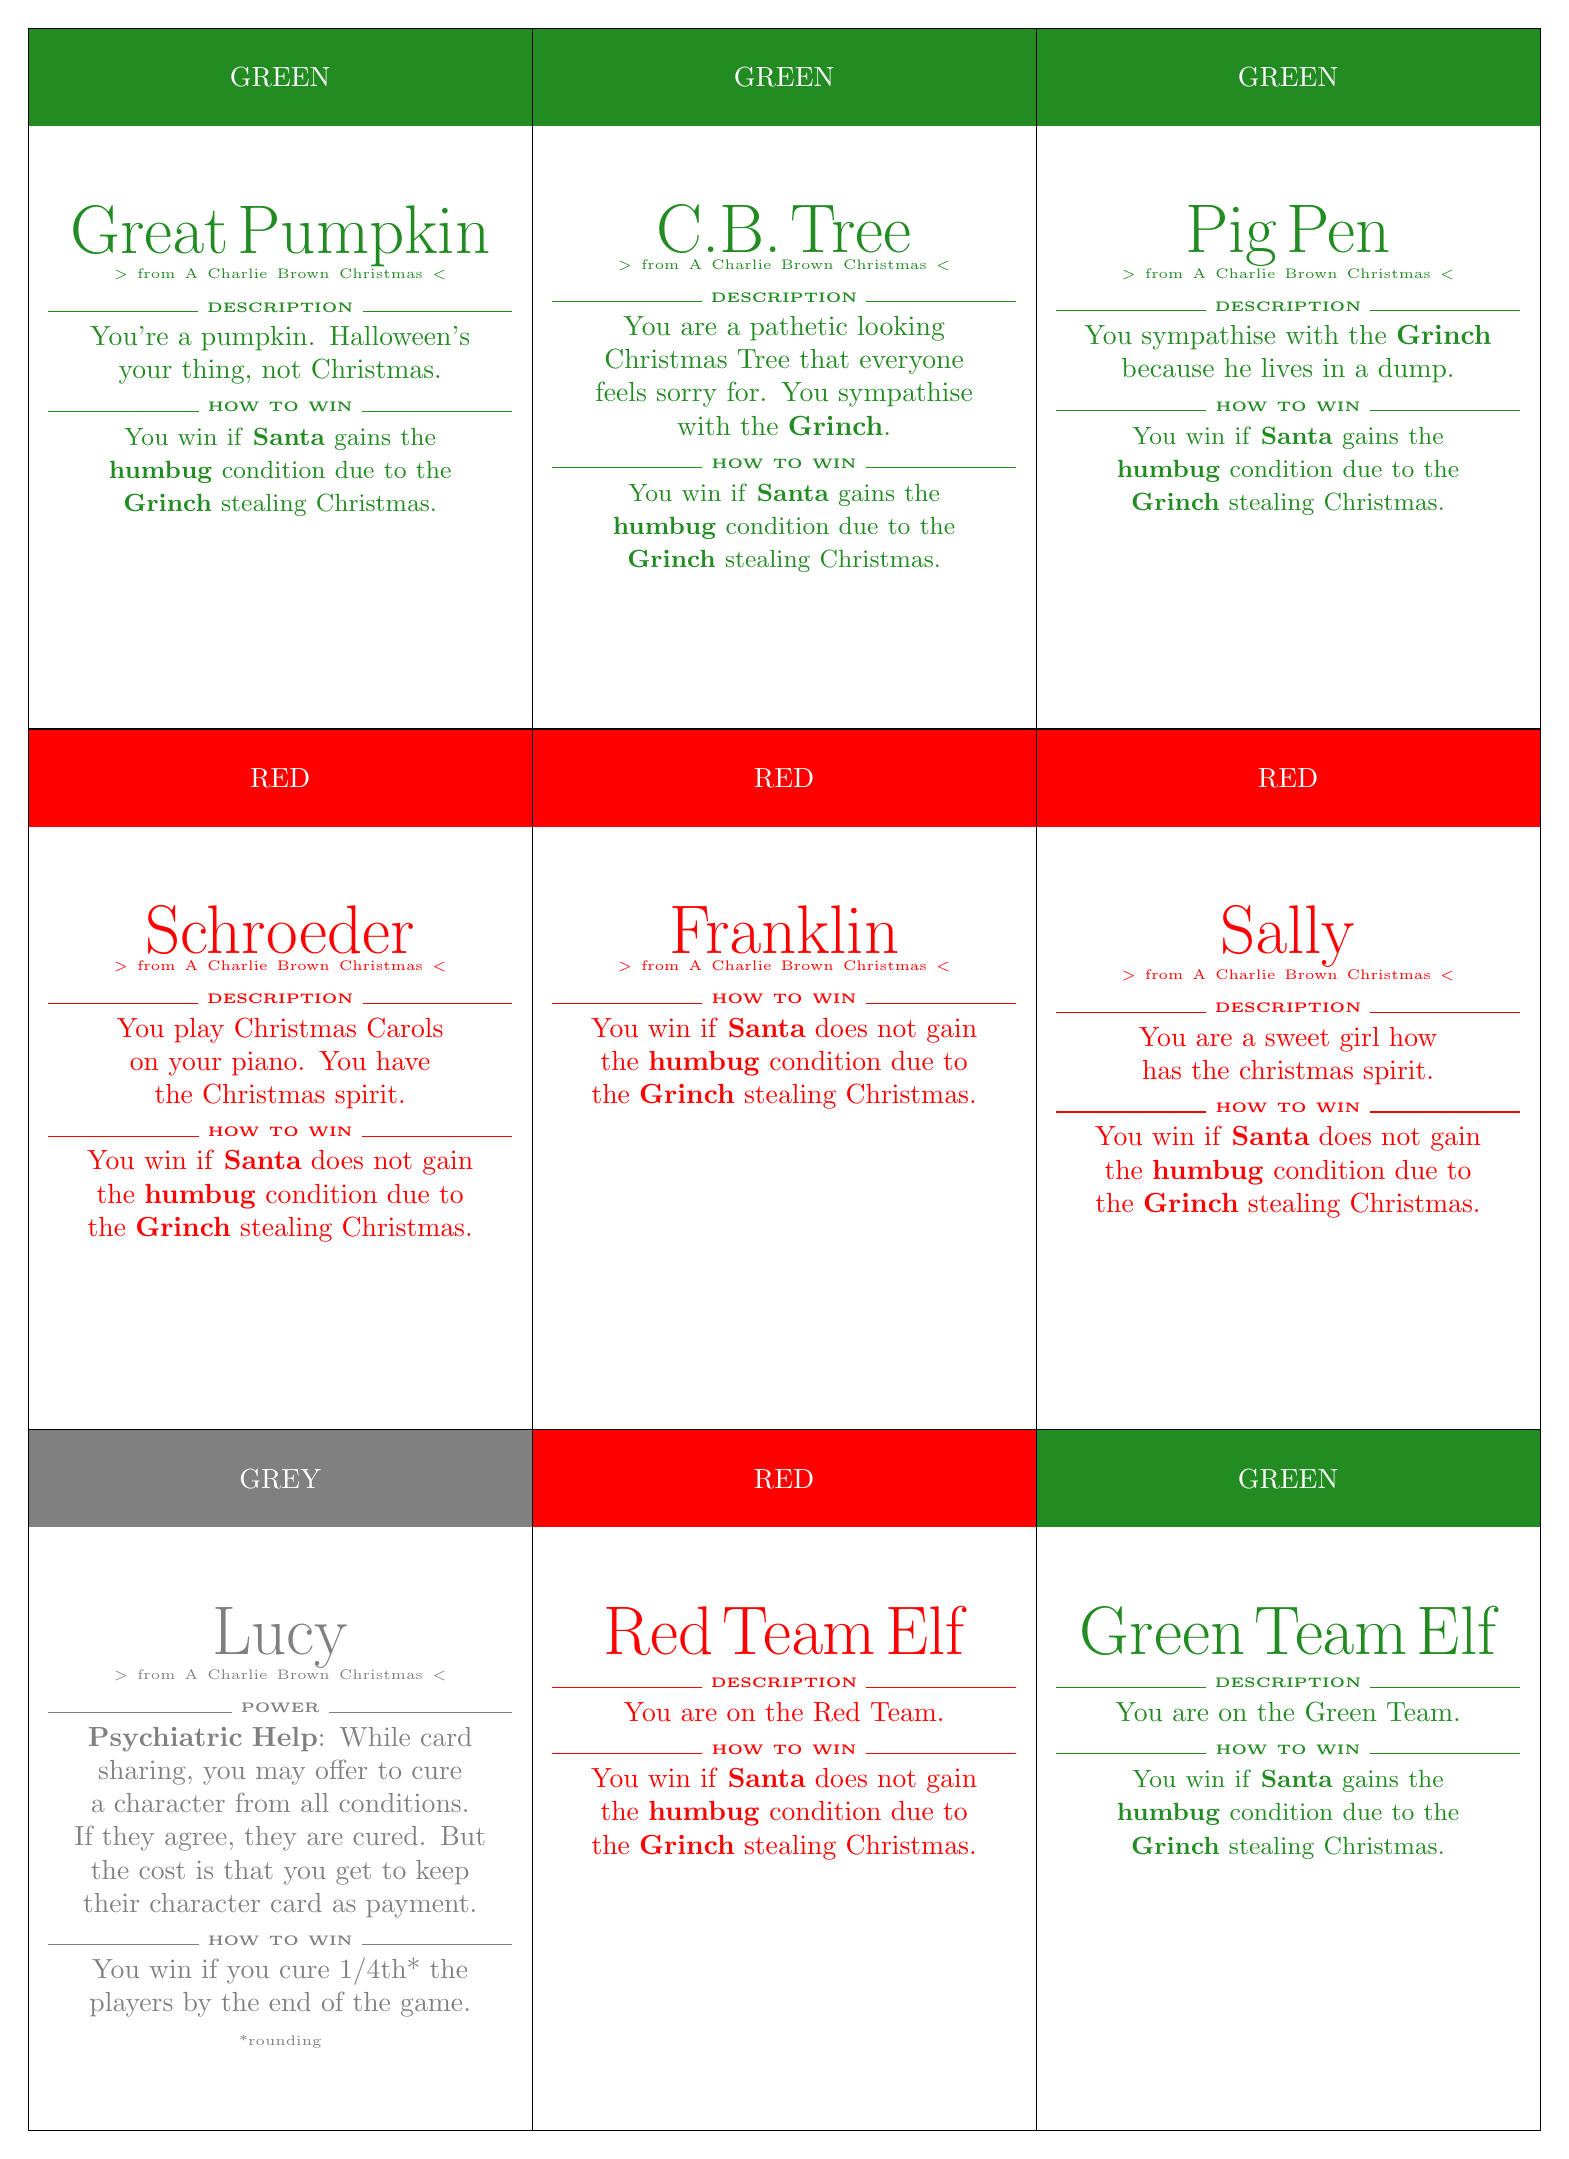
\begin{tikzpicture}[outer sep=0]

% THE GREAT PUMPKIN
\node[teamshare, fill=ForestGreen] (1) at (3.2,26.7) {\HUGE GREEN};
\node[cardtext, text=ForestGreen] at (3.2,24.7) {
	{\Huge Great Pumpkin}
	\titlefrom{A Charlie Brown Christmas}
	\seperatordescription
	You're a pumpkin. Halloween's your thing, not Christmas.
	\greenwinsection
};

% CHARLIE BROWN CHRISTMAS TREE
\node[teamshare, fill=ForestGreen] at (9.6,26.7) {\HUGE GREEN};
\node[cardtext, text=ForestGreen] at (9.6,24.7) {
	{\Huge C.B. Tree}
	\titlefrom{A Charlie Brown Christmas}
	\seperatordescription
	You are a pathetic looking \\ Christmas Tree that everyone\\ feels sorry for. You sympathise \\with the \character{Grinch}.
	\greenwinsection
};

% PIG PEN
\node[teamshare, fill=ForestGreen] at (16,26.7) {\HUGE GREEN};
\node[cardtext, text=ForestGreen] at (16,24.7) {
	{\Huge Pig Pen}
	\titlefrom{A Charlie Brown Christmas}
	\seperatordescription
	You sympathise with the \character{Grinch} because he lives in a dump.
	\greenwinsection
};

% SCHROEDER
\node[teamshare, fill=red] at (3.2,17.8) {\HUGE RED};
\node[cardtext, text=red] at (3.2,15.8) {
	{\Huge Schroeder}
	\titlefrom{A Charlie Brown Christmas}
	\seperatordescription
	You play Christmas Carols \\on your piano. You have the Christmas spirit.
	\redwinsection
};

% FRANKLIN
\node[teamshare, fill=red] at (9.6,17.8) {\HUGE RED};
\node[cardtext, text=red] at (9.6,15.8) {
	{\Huge Franklin}
	\titlefrom{A Charlie Brown Christmas}
	\redwinsection
};

% SALLY
\node[teamshare, fill=red] at (16,17.8) {\HUGE RED};
\node[cardtext, text=red] at (16,15.8) {
	{\Huge Sally}
	\titlefrom{A Charlie Brown Christmas}
	\seperatordescription
	You are a sweet girl how has the christmas spirit.
	\redwinsection
};

% LUCY
\node[teamshare, fill=gray] at (3.2,8.9) {\HUGE GREY};
\node[cardtext, text=gray] at (3.2,6.9) {
	{\Huge Lucy}
	\titlefrom{A Charlie Brown Christmas}
	\seperatoraction
	\condition{Psychiatric Help}: While card sharing, you may offer to cure a character from all conditions. \\
	If they agree, they are cured. But the cost is that you get to keep their character card as payment.
	\seperatorwin
	You win if you cure 1/4th* the players by the end of the game. \\
	\tiny *rounding
};

% RED TEAM ELF
\node[teamshare, fill=red] at (9.6,8.9) {\HUGE RED};
\node[cardtext, text=red] at (9.6,6.9) {
	{\Huge Red Team Elf}
	\seperatordescription
	You are on the Red Team.
	\redwinsection
};

% GREEN TEAM ELF
\node[teamshare, fill=ForestGreen] at (16,8.9) {\HUGE GREEN};
\node[cardtext, text=ForestGreen] at (16,6.9) {
	{\Huge Green Team Elf}
	\seperatordescription
	You are on the Green Team.
	\greenwinsection
};


\draw (0,0) -- (19.2,0);
\draw (0,8.9) -- (19.2,8.9);
\draw (0,17.8) -- (19.2,17.8);
\draw (0,26.7) -- (19.2,26.7);

\draw (0,0) -- (0,26.7);
\draw (6.4,0) -- (6.4,26.7);
\draw (12.8,0) -- (12.8,26.7);
\draw (19.2,0) -- (19.2,26.7);



\end{tikzpicture}

%Background is not my own. But courtesy of a user on BGG

\includepdf[pages={1}, angle=90]{cardsbackground.pdf}


\end{document}